\documentclass[sigconf]{acmart} 

%\usepackage{booktabs} % For formal tables
%\usepackage[utf8]{inputenc}
\usepackage{graphicx}
\usepackage{float}
%\usepackage{cite}
\usepackage{subcaption}
\usepackage{tcolorbox}
\setlength{\marginparwidth}{2cm}  % for todo notes
\usepackage[colorinlistoftodos]{todonotes} % handig voor commentaar: gebruik \todo{}, zie ftp://ftp.fu-berlin.de/tex/CTAN/macros/latex/contrib/todonotes/todonotes.pdf
%\usepackage{listings}
% linenumbering  See https://texblog.org/2012/02/08/adding-line-numbers-to-documents/
\usepackage{lineno}
\linenumbers

% Copyright
\setcopyright{none}

\title{Armchair Auditing of Insolvency Processes}
\author{Tom Akkermans}
\affiliation{\institution{University of Amsterdam}}
\email{tom.akkermans@student.uva.nl}
\acmConference[University of Amsterdam]{2}{3}

\begin{document}

\begin{titlepage}
\begin{center}

\textsc{\Large Data Driven Supervision in Insolvency Procedures }

\bigskip

\textsc{\large
submitted in partial fulfillment for the degree of master of science\\
%
\bigskip
Tom Akkermans\\
%
11323671\\
%
\bigskip
master information studies\\
%
data science \\
%
faculty of science\\
%
university of amsterdam\\
%
\bigskip
%Your Date of defence in the format YYYY-MM-DD
2018-08-18
}

\end{center}
 

\vfill

% In case of an internal project, remove External Supervisor or if you had two internal supervisors, change the header into 
%  & First Supervisor & Second Supervisor  \\
\begin{center}
\begin{tabular}{|l||ll|}
\hline
 & \textbf{First Supervisor} & \textbf{Second Supervisor}  \\   
 \hline
\textbf{Title, Name} & Dr Maarten Marx&  \\
\textbf{Affiliation} &UvA, FNWI, IvI & \\ 
\textbf{Email} & maartenmarx@uva.nl& . \\
\hline
\end{tabular}
\end{center}

\bigskip

% logos
\begin{center}
\mbox{
\includegraphics[width=.2\paperwidth]{logo-uva.png} 

\includegraphics[width=.2\paperwidth]{ads.png}
}
\end{center}
\end{titlepage}

%
%\newpage
%
%\end{document}

\maketitle 

% \begin{abstract}
When a company is declared bankrupt by the court, a court committee appoints a administrator to settle the bankruptcy. The administrator's task is to cash in the company's estate and use it to settle the creditors claims. A court's judge must supervise the administrator in order to to act in the best interest of the creditors.

The supervisory function of the judge, the conflict of interest between the administrator and creditors and the appointment process of the administrator are processes which have been the subject of research\cite{boluk_2011}, about which media articles have appeared \cite{dennis_meneer_2018:1, dennis_meneer_2017:1, jan-hein_strop_2015:1} and which have led to legal proceedings. The involved parties ask for more transparency and information about these processes. Access for the general public and journalists to this process information could provide an extra check and thus further improvement of processes.

The Dutch government started in 2005 publishing insolvency data\cite{rechtspraak:1} according to the insolvency law \cite{law:1}. It provides an on-line search form to retrieve a single insolvency case and provides open data sources with technical APIs that provide court publications and administrator reports. However, the information from a single insolvency case is limited, the report information is unstructured and not all interested parties can deal with the raw data APIs. Instead of open data, there is a need for open analysis to enable an 'armchair audit'\cite{o_leary_2015} of insolvency processes to answer their questions.

In this thesis a prototype of an information system will be presented that enables the audit of insolvency processes for non-technical stakeholders. The system processes large amounts of structured and unstructured data of insolvency processes using open and publicly available data sources. From this data, the system builds and annotates a fully linked, clean entity structure of insolvents, administrators, judges, courts as well as administrator reports and court publications. Unstructured administrator report data is made searchable at multiple levels and process data is uncovered. 

We describe the implementation challenges and show that the system can provide new insights to the interested party who can use a non-technical interface to investigate the insolvency processes and answer specific questions. 
\end{abstract}


% The code below should be generated by the tool at
% http://dl.acm.org/ccs.cfm
% Please copy and paste the code instead of the example below.
%
%\begin{CCSXML}
%<ccs2012>
%	<concept>
%		<concept_id>10002951.10003317.10003347.10003349</concept_id>
%		<concept_desc>Information systems~Document filtering</concept_desc>
%		<concept_significance>300</concept_significance>
%	</concept>
%</ccs2012>
%\end{CCSXML}
%\ccsdesc[300]{Information systems~Document filtering}

%\keywords{[todo]}

\section{Introduction}
When a company is declared bankrupt by the court, a court committee appoints an administrator to settle the bankruptcy. The administrator's task is to liquidate the company's estate and use the proceeds to settle the creditors claims. A supervisory judge ensures that the administrator is acting in the best interest of the creditors. 

Involved parties have been demanding more transparency into insolvency processes. The supervisory function of the judge, the conflict of interest between the administrator and creditors and the appointment process of the administrator are processes which have been the subject of research\cite{boluk_2011}, about which media articles have appeared \cite{dennis_meneer_2018:1, dennis_meneer_2017:1, jan-hein_strop_2015:1} and which have led to legal proceedings. \todo{citeer}  

\begin{comment}
Other benefits: Supervisory judges with significant work load could benefit from data driven supervision. Information access to the general public and journalists to this processes  would provide additional checks and balances.
\end{comment}

In 2005 the Dutch government started the digital register of insolvency data\cite{rechtspraak:cir}. An on-line search form \cite{rechtspraak:cir-zoeken} is provided to retrieve a single insolvency case. Web services are provided to retrieve court publications in XML format and administrator reports in PDF format. 

However, the information from a single insolvency case is limited as it does not provide aggregated and linked information. The administrator reports are unstructured and not searchable as a collection. Furthermore most involved parties lack the technical skills to use the web services. Instead of open data, there is a need for \textbf{open analysis} to enable 'armchair audits'\cite{o_leary_2015} of insolvency processes.

% main research question
In this thesis we investigate whether [RQ] \textbf{it is possible to build a complete and correct structured information system (IS) based on provided and enriched open and public data that is able to provide the requested transparency to the parties involved}.

For this we need to answer the following questions:
\begin{itemize}
	\item [RQ1] Can the IS construct a complete, cleaned and fully linked entity network of insolvency cases, administrators, judges and courts.
	\item [RQ2] Can the IS correctly and completely label insolvency case data with state data [start/end date] in order to mine the insolvency process.
	\item [RQ3] Can the IS correctly extract specific fields [paulianeus handelen] of interest from unstructured documents to classify insolvency cases.
	\item [RQ4] Can involved stakeholders use the IS to provide the requested transparency on insolvency processes.
\end{itemize}

We describe the steps in building such a system that takes in large amounts of open and publicly available data in structured and unstructured form, extracts and enriches useful facts and makes it consumable for analysis to provide insights into the insolvency processes via a web GUI.

\section{Information System Overview}
\subsection{System components}
Figure \ref{System overview} gives an overview of the system components for sourcing, extracting, enriching and integrating the  data and making the resulting structured and higher level information available to the user's analysis.

\begin{figure}[h]
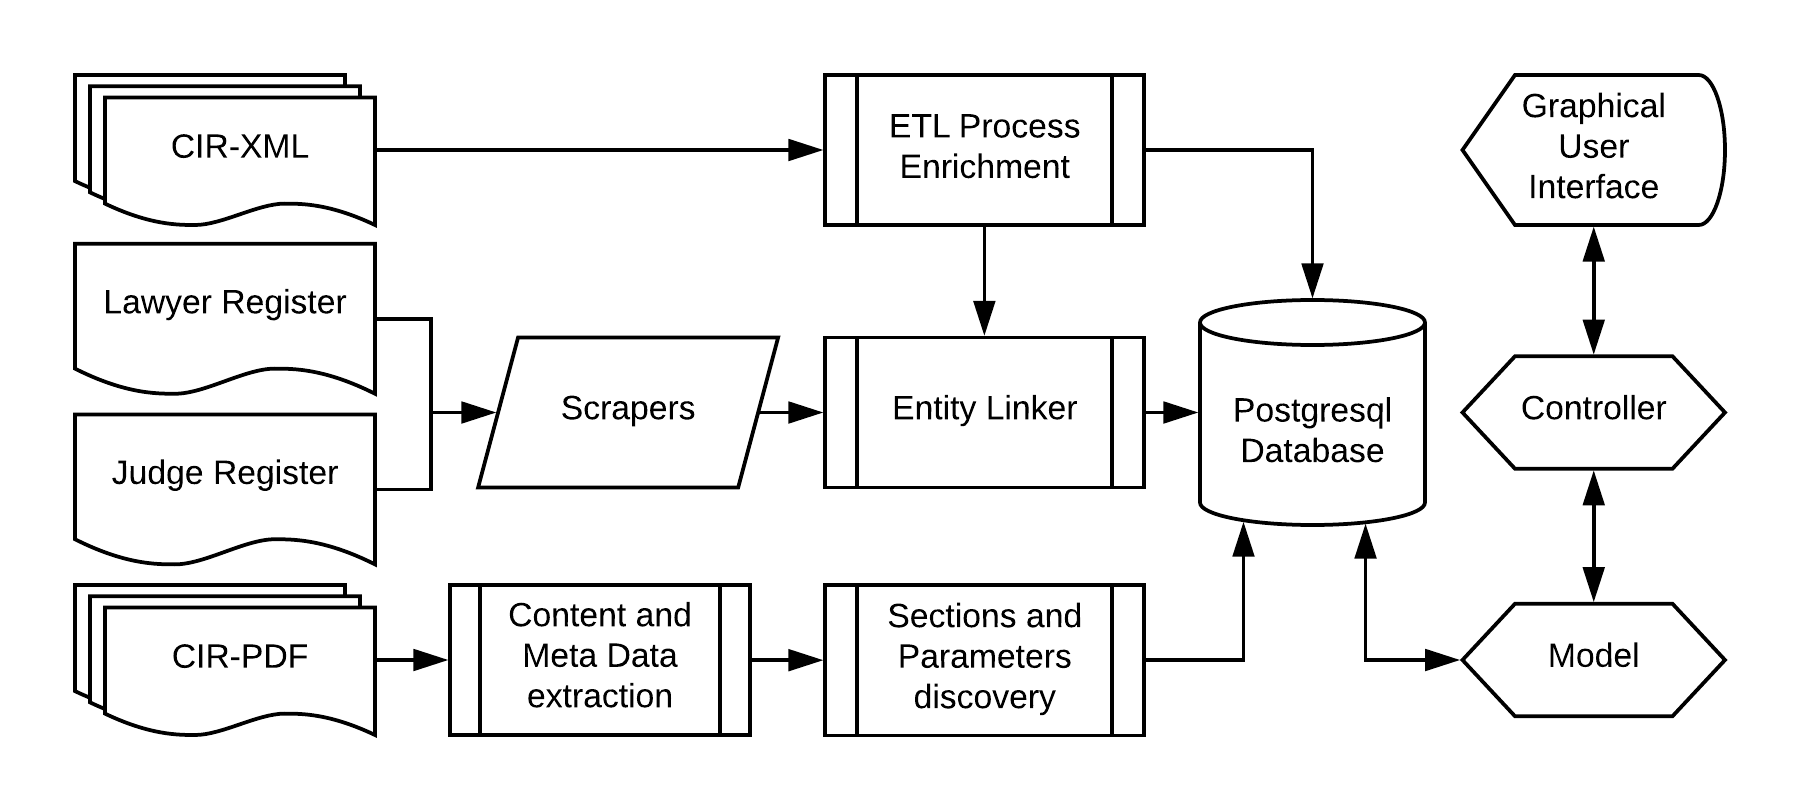
\includegraphics[width=1\linewidth]{images/system_overview.png}
\caption{System overview.}\label{System overview}
\end{figure}

Data flows from left to right through the following components:
\paragraph{Data Sources} Data is sourced from three public registers:
\begin{enumerate}
	\item The Central Insolvency Register (\textit{Centraal Insolventie Register or CIR}). CIR exposed both an XML and PDF file web service.
	\item The Register of lawyers (\textit{NOvA's Tableau}).
	\item The Register of ancillary positions of judges. (\textit{Register van nevenfuncties van rechters}) 
\end{enumerate}
The CIR provides the bulk of the data. The other two registers are used for the entity resolution of administrators and judges.

\paragraph{The ETL process and Enrichment} This component loads entities with selected data fields from the CIR XML data. The data is cleaned and enriched after which it is stored in a relational Postgresql database.

\paragraph{The Entity Linker} This component is responsible for linking judges and administrators in the CIR XML data to real life entities found in the judge and lawyer registers. 

\paragraph{PDF processors}
These component processes the CIR PDF reports to extract textual content and meta data. The text sections as defined in the progress report template and key data parameter are discovered in a subsequent process and loaded into the (Postgresql/Elastic) database.

\paragraph{Model-View-Controller (MVC)}
This well established pattern of subcomponents works together as a graphical interface for the user to analyse the data. 
%The user operates a graphical interface, prototyped in Jupyter notebooks, to query the data or interact with data visualisations or tables. The interface is the View in the MVC component. On user command, the Controller asks the Model to prepare the necessary data and then passes this data to the View to update the interface.

\subsection{Description of data sources}
\subsubsection{Central Insolvency Register}
\paragraph{Data suppliers}
The CIR \cite{rechtspraak:1} is operated by the state and contains company insolvency data supplied by the courts and the administrators. Courts are obliged to supply the insolvency data and free consultation thereof according to the insolvency law, article 19 \cite{law:1}. CIR started the register on the 1st of January 2005 and retains insolvency cases until six months after the ending of the insolvency.

\paragraph{Entities}
CIR data contain the following entities:

\begin{itemize}
	\item Courts
	\item Court Publications
	\item Supervisory Judges 
	\item Insolvency Cases
	\item Administrators
	\item Administrator Reports
\end{itemize}

\begin{figure}[h]
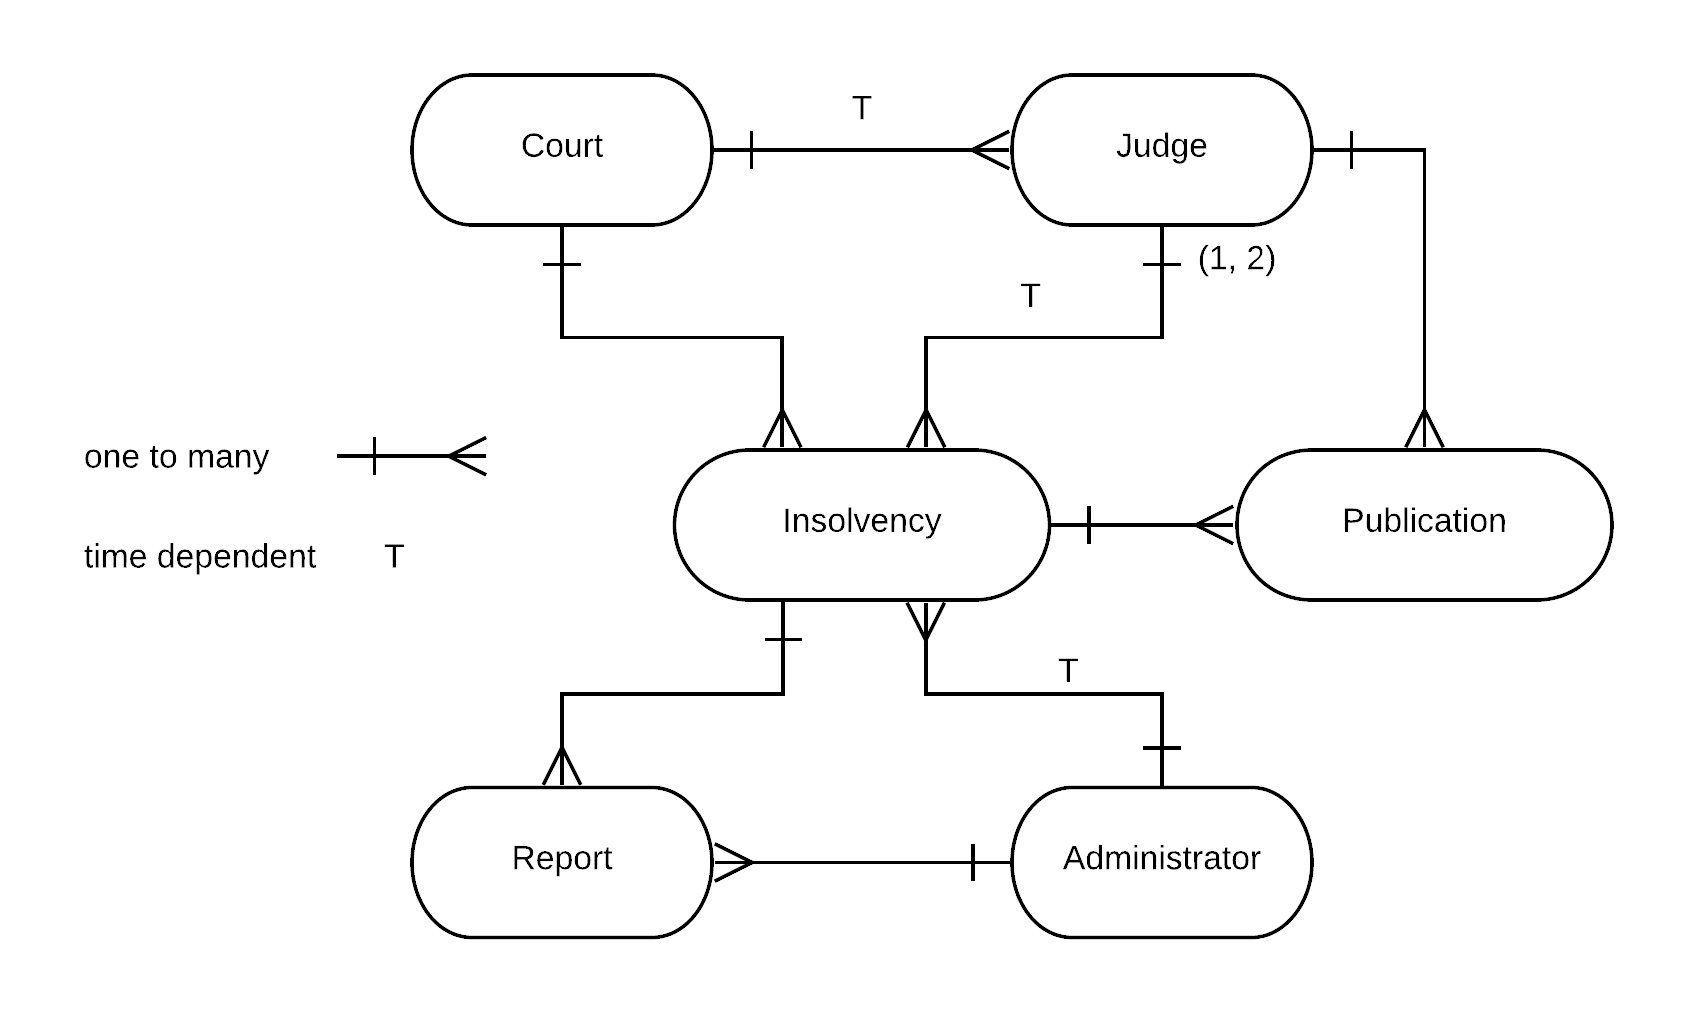
\includegraphics[width=1\linewidth]{images/cir_erd_2.png}
\caption{Insolvency entity relations.}
\end{figure}
\todo[inline]{remove law firm if not relevant. rename insolvent to insolvency}

\paragraph{CIR data contents}
Table \ref{table:cir_contents} shows the content of the CIR register data as of date [2018-08-12] and the average monthly size of new additions.

\begin{table}[h]
\caption{number of entity records and avg. monthly growth.}
\centering
\begin{tabular}{l r r}
\hline\hline
Entity & no. of records & delta\\
\hline
Insolvency & 17,331 & 280 \\
Report & 146,865 & 4408 \\
... progress report & 87,430 &  \\
... financial attachment. & 56,611 &  \\
Publication & 37,031 & 1447 \\
Administrator (distinct names) & 2329 & \\
Judge (distinct names) & 451 & \\
Court & 11 & \\
\hline
\end{tabular}
\label{table:cir_contents}
\end{table}
\todo[inline]{update numbers}

\paragraph{Identifiers}
The web service response in XML is semi structured data. It provides unique identifiers for Insolvency Cases, Publications and Reports	which can be stored in normalized SQL tables. The other entities Courts, Judges and Administrators have no identifiers but consist of free text fields for their name parts. These entities must be de-duplicated en linked to a real world entity.

\paragraph{Administrator Reports}
A second web service operated by CIR provides Administrator Reports in PDF format that hold much of the unstructured data. There are two types of reports: 
\begin{enumerate}
\item progress reports
\item financial attachments
\end{enumerate}
Recofa has published templates for both report types\cite{rechtspraak:3}.


\subsubsection{Register of lawyers, NOvA Tableau}\label{NOvA Tableau}
The NOvA tableau is the official register for lawyers and maintained by the \textit{Nederlandse Orde van Advocaten (NOvA)}\cite{nova:1}. Lawyers are obliged to be registered in the tableau by the lawyer's law (\textit{advocatenwet}, article 1 \cite{law:2}). NOvA offers an on-line search form where key word search and filters can be applied to search for a lawyer. This data source is used to collect the master data for Administrators. 

\subsubsection{Register of judges, Nevenfuncties van rechters}\label{Nevenfuncties Rechters}
The Register for ancillary positions for judges is made available by \textit{de Rechtspraak}\cite{rechtspraak:2}. It offers an on line form and returns the name, current and historical occupation and ancillary positions. This data source is used to collect the master data for Judges.
% \section{Related Work}
\todo[inline]{add related work on entity linking, deduplication etc}

\subsection{Research Questions}
The main research question is:
\textbf{Is is possible to build a useful, complete and correct structured information system based on unstructured CIR data?}

The system is build on three components
\begin{itemize}
\item extraction of insolvency process flow information.
\item construction of a fully linked, clean entity structure of insolvents, administrators, judges, courts as well as administrator reports and court publications.
\item extraction the text and parameters in administrator reports and indexes sections and parameters by imposing structure on the content.
\end{itemize} 

\begin{itemize}
\item \textbf{useful}: the system is useful when it can answer questions of the parties involved or can answer these questions much more efficient than with current methods. We define so-called Persona to represent archetypical users of the information system and define specific questions they have. These questions are distilled from the insolvency law, news articles, research papers, court cases [refs] and interviews. [How do we measure, which section]
\item \textbf{complete} the system's entity structure is complete when all main entities and their inter relations are found. Completeness is also defined for specific parameters needed to answer the user's questions. [How do we measure, which section]
\item \textbf{accuracy} The system's identity structure is accurate when entities refer to their actual real life counterparts. The [How do we measure, which section]


\end{itemize}


% \section{Methodology}
\input{chapters/methodology-data-sources}

\paragraph{Database normalization}
This leads to unwanted duplication as names can be written in many different forms and typos can be introduced, e.g. one judge's name appears as:

\begin{itemize}
\item "mr. W.J. Geurts - de Veld"
\item "mr. W.J. Geurts-deVeld"
\item "mr. W.J. Geurts-de Veld"
\item "mr. W.J.Geurts-de Veld"
\item "mr.W.J. Geurts-de Veld"
\item "mr. W.J. Geurts-de Veld (Rotterdam)"
\item "mr W.J.Geurts-de Veld"
\item "W.J.Geurts-de Veld"
\end{itemize}

We need to define so-called master data for judges and administrators containing the real world entities. The two data sources in the sections \ref{NOvA Tableau} and \ref{Nevenfuncties Rechters} are chosen for this purpose. CIR entity names are first normalized for de-duplication and are subsequently linked to the master data records on their normalized name. 

\paragraph{PDF report web service}




The number of current defaults is about the lowest of the century [ref] [graph of declining defaults]






\subsection{Implementation challenges}
\subsubsection{Entity De-duplication, Scraping and Linking}
\paragraph{Deduplication: normalizing names}
CIR provides administrator names in four parts: title, initials, middle part and family name. 

\textbf{The initials} were normalized into single characters using periods and no spaces. In Dutch, initials for names like \textit{Theodoor} and \textit{Christiaan} are written with two or three characters as \textit{Th.} or \textit{Chr.}. These names are derived from the Greek where the initial \textit{Th(eta)} for example is written as one character. Initials for double names like \textit{Albert-Jan} may be written as \textit{A-J.} or \textit{A.-J.}. 

\textbf{The middle part}, e.g. 'van der' or 'ter' was sometimes supplied in the middle part field and sometimes in the family name (and sometimes in both). To normalize the middle part it was merged into the family name making sure it did not appear twice.

\textbf{The family name} was stripped from academic and noble (not uncommon in this profession) titles. Misplaced initials and CIR specific comments were removed. Maiden names are connected to the surname with a hyphen and no spaces.

Furthermore, all parts are made lower case, surrounding whitespace characters are stripped, accents are removed and multiple spaces are replaces with a single space. 

De-duplication by normalizing the administrator names reduced the number of distinct administrator names from 2329 to 1559, a 33\% reduction.
\\\\
Judge names are provided in a single field. This sometimes leads to initials or a middle name part that is stuck together to the family name and was separated using regexm e.g. in 'C. vanSteenderen' and 'mr. W.J.Geurts-de Veld'. CIR often adds the court between parenthesis which was also removed in the normalization.

De-duplication by normalizing the judge names reduced the number of distinct judge names from 565 to 277, a 51\% reduction.

\paragraph{Administrator name scraping}
NOvA unfortunately does not provide complete lists of registered lawyers to which we could link the administrators. Instead we link the administrator by using the site's search form. An underlying REST API returning JSON data was discovered which was used instead of the form. The API (or form) can not handle initials or stop words as 'de' and 'van' and only the family name without stop words was used. The best candidate in the search results, which are sorted on the relevance provided by NOvA, is found by (partially) matching the initials until a match is found. The API enables the use of filters and we filter from narrow to broad until a candidate is found, filtering on: 
\begin{enumerate}
\item{legal specialism: administrator}
\item{legal branch: insolvency law}
\item{no filter}
\end{enumerate}

NOvA only supplies the actual lawyer register but CIR also lists administrators previously working on a case therefore a substantial amount of administrators cannot be linked. Another website, www.advocatenzoeken.nl that sources data from NOvA but keeps historical data was scraped as well to complement NOvA.

\paragraph{Administrator name linking}
From the normalized name list we linked 73\% to NOVa registered lawyers and another 18\% administrators from the www.advocatenzoeken.nl site. The remaining 10\% unfound names are linked to a special 'unknown' lawyer.

\begin{table}[h]
\caption{Administator entity linking results}
\centering
\begin{tabular}{l r r r}
\hline\hline
Source & no. linked & correct & incorrect\\
\hline
NOvA & 1134 & 1133 & 1\\
AdvocatenZoeken & 280 & 279 & 1 \\
Not found & 149 &&\\
\hline
Total & 1563 & 1412 &\\
\hline
\end{tabular}
\label{table:administrator_linking}
\end{table}

Correctness is assumed when the names match. When an obvious typo is found in the family name. When the initials either match, or are contained in the master record or are permutated or are missing. 

[discuss not found results: common name, place in name]

\paragraph{Judge name scraping}
The CIR register for ancillary functions for judges was scraped for judges from courts and higher courts. The total set contains 3691 judges and should be a superset of active case judges. The website was driven by the Angular javascript framework and could not easily be scraped with simple HTTP requests. Selenium was used to mimic user browsing behaviour to invoke the javascript. 

\paragraph{Judge entity linking}
A judge is linked by to a judge master record with the most similar normalized name where similarity was calculated using the Levensthein or edit distance. 88\% of the normalized names were matched. 4 of the incorrectly 12\% matched names could be set manually and the remaining 8\% was linked to a special 'unknown' judge.


\begin{table}[h]
\caption{Judge entity linking results}
\centering
\begin{tabular}{l r r r}
\hline\hline
Source & no. linked & correct & incorrect\\
\hline
Ancillary positions register & 277 & 246 & 32\\
+Manual lookup of the 32 &   & 10 & -10\\
\hline
Total & 277 & 256 & 22\\
\hline
\end{tabular}
\label{table:judge_linking}
\end{table}

Correctness is defined similar to the administrator normalized name correctness.

[discuss not found (initially) results: maiden name, not a judge anymore]

\subsubsection{Process Mining}

\subsubsection{PDF content extraction}
The PDF reports can be split into two types depending on how the PDF was created:
\begin{enumerate}
\item Scanned from paper using a scanner or copier.
\item Converted by software from another format.
\end{enumerate}

\paragraph{Scanned PDFs}
Scanned PDFs contain images only. To convert the images to text we used the Ghostscript library for image extraction and the Tesseract OCR engine for the character recognition. Tesseract supports the Dutch language which is paramount to our application. It is very important to supply Tesseract with good quality images. We used the Ghostscript settings of a \emph{tiffgray} output device with a \emph{300 DPI} resolution. 

\paragraph{Converted PDFs}
Converted PDF content can be extracted with a number of packages such as PDFMiner, PyPDF2, pyPoppler and pdftotext. We chose the latter after comparison because it maintains the layout which is important for section and parameter extraction and being build in C++ it is very fast.

\paragraph{Third type}
A third type appeared: PDFs that were scanned and subsequently OCR-ed by a copier. They contain both text and images. The OCR quality is often poor. We retried re-OCR-ing the images with Tesseract which solved some errors but introduced others. Meta data about a.o. the scanner type was obtained which could improve post-process text extraction in future work.


\subsubsection{PDF report section and parameter extraction}
[todo]




\input{chapters/entity_resolution}
% \section{Evaluation}

%dedup lawyers: Phonetic similarity
%https://www.quora.com/What-is-a-good-algorithm-service-for-fuzzy-matching-of-companies-names-for-de-duplication


%\section{Conclusions}
%\subsection{Acknowledgements}

\bibliographystyle{ACM-Reference-Format}
\bibliography{bibliography}  
% \section{Appendix: Persona}
The main Persona are: 
\begin{itemize}
\item \textbf{The Judge} representing the side of Recofa, \textit{Raad van de Rechtspraak} and The Bankruptcy Judge (\textit{Rechter-Commissaris})
\item \textbf{The Administrator} representing the side of Insolad (Vereniging Insolventierecht Advocaten) and The Administrator (Curator) 
\item \textbf{The Insolvent} representing the owner(s) of the defaulted company.
\item \textbf{The Creditor} representing the Unsecured Creditor (\textit{De Concurrente Schuldeiser}).
\item \textbf{The Journalist} representing the investigative and economic journalist.
\end{itemize}

In the following sections each Persona will be described and their questions to the system stated.

\subsection{The Judge}
The Persona of Judge is interested in the adherence to the insolvency law and to the Recofa policy guidelines. It is also interested in specific trends in the insolvency processes and operational issues such as work pressure for judges. On an individual judge level it is interested in supervising its active cases.

Questions:
\begin{itemize}
	\item How many cases does a judge supervise at a certain point in time (now)
	\begin{itemize}
		\item … distribution over all judges at a certain court
		\item … distribution over all judges at all courts
	\end{itemize}
	\item What is the process flow of cases through court: 
	\begin{itemize}
		\item What is the case time distribution from begin to end
		\item How long does it take to set the verification meeting (law says < 14 days)
		\item How long does it take to publish the plan of final distribution.
		\item What percentage of cases:
		\begin{itemize}
			\item end early as there are no assets
			\item end by paying all creditors
			\item contain an agreement between insolvent and creditors (akkoord)
			\item are following an simplified settlement (no meeting of creditors)	
			\item are filed by the insolvent vs creditor
		\end{itemize}
		\item What are the experience factor (\textit{jaren praktijkervaring}) and estate factor (\textit{grootte actief}) for the cases determining the administrators hourly wage.
	\end{itemize}
	
	\item Are administrators reporting according to the instructions:
	\begin{itemize}
		\item How often is the progress reporting deadline breached.
		\item How often is the financial attachment omitted for all reports in a case.
	\end{itemize}
	\item Are administrators using the supplied template for progress report:
	\item How often does insolvency fraud occur
	\item \textit{What are the issues in progress reports that need the judge's attention}
\end{itemize}

\subsection{The Administrator}
The Persona of Administrator is interested in the administrator appointment process of the courts and on issues that threaten its business or leave it powerless.\\

from \cite{samr_2017:1}:\\
\textit{"Volgens de curatoren is meer transparantie van belang
bij de verdeling van faillissementen: ze ervaren deze
verdeling nu als een black box. [...] Daarnaast maken de curatoren
zich flinke zorgen over het hoge verloop onder rechtercommissarissen
en de griffie en de gevolgen daarvan."}\\

Questions:
\begin{itemize}
	\item Which curators are on the court’s short list for appointment
	\item Are insolvency cases distributed fairly over the curators on the list
	\item How long are judges working in the insolvency field, how often do they rotate.
	\item How often do empty estates occur (an empty estate implicated work without pay)
	\item To what degree do Banks claim all the proceeds from the assets.
\end{itemize}

\subsection{The Insolvent}
The Persona of Insolvent could be interested in restarting the business. It also is afraid of being made personally liable for the bankruptcy claims.

\begin{itemize}
	\item -	How often are insolvent made personally liable (when there is little estate)
	\item -	How often do insolvency restarts and prepacks occur
\end{itemize}

\subsection{The Creditor}
The Persona of Creditor is interested in the recovery rate of its claim and the time of payout and the factors that influence those.

\begin{itemize}
	\item What is my expected recovery rate and time
	\item -	How high is the administrator’s salary, is he eating up the proceeds.
\end{itemize}

\subsection{The Journalist}
The Persona of Journalist is writing an article on a certain insolvency phenomenon. An economic journalist might periodically write the same story on say the number of defaults in the last quarter compares to a previous period, usually for business readers. The investigative journalist writes for a wide audience, therefore the article contains both general trends as well as the personal individual story. For this the investigative journalist needs query functionality to dig for evidence and pull individual records.

\begin{itemize}
	\item J2: (topic: incapable administrators) Which administrators have often been taken of their cases by the judge.
	\item J1: How many defaults occurred over the last three months compared to a year earlier. [viz:cumulative lines of two periods]
\end{itemize}

\end{document}

